\documentclass[a4paper]{article}
\usepackage[utf8]{inputenc}
\usepackage{graphicx} % Required for inserting images
\usepackage[italian]{babel}
\usepackage{gensymb}
\usepackage{array}
\usepackage{amsmath}
\usepackage{hyperref}
\usepackage{siunitx}
\usepackage{caption}
\usepackage{placeins}
\usepackage[margin=3cm]{geometry}

\makeindex
\setlength{\parindent}{0pt}

\title{Misura del Calore Specifico di un Solido e del Calore Latente del Ghiaccio}
\author{Francesco Giuliano Rossi}
\date{Maggio 2025}
\begin{document}
\maketitle
\tableofcontents

\begin{abstract}
    L'obbiettivo di questo sperimento, diviso in tre parti, è di verificare il valore teorico per la massa equivalente in acqua, il calore specifico di un materiale (in questo caso ottone) e il calore latente del ghiaccio. Attraverso la misura della temperatura, e conoscendo la massa, si possono ricavare tutti i valori. 
\end{abstract}

\section{Introduzione Teorica}
\subsection{Calorimetro delle Mescolanze}
Uno degli apparati principali usati in questo sperimento è il calorimetro di Regnault, o anche delle mescolanze. Questo apparato è costituito da un vaso calorimetrico, circondato da pareti adiabatiche a doppio strato, riflettenti, dove in mezzo ai due strati c'è il vuoto. In questo modo si riduce il più possibile lo scambio di calore con l'ambiente. Inoltre, è presente un agitatore, in questo modo non è necessario tenere conto della differenza di temperatura in punti diversi perché ogni punto avrà la stessa temperatura. All'interno del calorimetro, possiamo misurare delle quantità di calore, attraverso la relazione $Q = C\Delta T$
dove $C$ è la capacità termica del sistema, $Q$ è una quantità di calore incognita e $\Delta T$ è la variazione di temperatura ad essa collegata. Mettendo quantità note di calore e misurando la variazione di temperatura, si può trovare la capacità termica $C$ del calorimetro.\\
Anche se molto bene isolato dall'esterno, l'apparato non può essere considerare un sistema termicamente isolato dall'ambiente. La legge che regola lo scambio di calore, se le temperature all'interno e quella dell'ambiente sono simili, si può approssimare a 
\begin{equation}
    dQ = \delta [T_A - T(t)]dt
\end{equation}
dove $\delta$ è la conducibilità delle pareti del calorimetro per conduzione e irraggiamento e tiene conto dell'evaporazione del liquido, $T_A$ è la temperatura dell'ambiente, e T(t) è la temperatura a un certo istante $t$. Ricordandosi che $dQ = CdT$, sostituendo e integrando, Segue che temperatura del sistema calorimetrico può essere descritta dalla legge esponenziale 
\begin{equation}
    T(t) = T_A + (T_0 - T_A) e^{-\frac{t}{\tau}}
\end{equation}
dove $\tau = \frac{C}{\delta}$ è la costante di tempo del calorimetro. Per tempi piccoli rispetti a $\tau$, si può fare un'espansione di Taylor del primo ordine, fermandoci al primo termine, e si ottiene che 
\begin{equation}
    T(t) = T_0 - \frac{(T_0 - T_A)}{\tau}t
\end{equation}
In questo modo, misurando un intervallo di tempo abbastanza grande, si riesce a vedere una differenza non trascurabile nelle temperature $T(t)$ e $T(t_0)$. Introducendo nel calorimetro una quantità nota di massa $m_1$, una volta raggiunto l'equilibrio termico con il calorimetro, si misura la temperatura $T_1$, e si aggiunge una seconda quantità di massa $m_2$, con temperatura $T_2 > T_1$. Raggiunto l'equilibrio a temperatura $T^*$, si avrà
\begin{equation}\label{eq}
    (m_1 c_a + C_c) (T^*-T_1) = m_2 c_a (T_2-T^*)
\end{equation}

\subsection{Massa Equivalente in Acqua}
Come già detto, non si può trascurare il fatto che il calorimetro non sia un sistema isolato. Tuttavia, trovare quanto esattamente contribuisce sarebbe difficile per la quantità di fattori che si deve tenere in conto. Per evitare di misurare tutte queste quantità, si preferisce esprimere questa quantità come una quantità equivalente di una sostanza, di cui si conoscono le caratteristiche. Questa quantità si chiama l'equivalenza in acqua del calorimetro
\begin{equation}
    C_c = c_am^*
\end{equation}
L'equazione \ref{eq}, così diventa 
\begin{equation}
    c_a (m_1+m^*)(T^*-T_1) = c_a m_2 (T_2-T^*) 
\end{equation}
Che non dipende dalla capacità termica specifica dell'acqua. Una volta raggiunta e misurata la temperatura di equilibrio $T^*$, si può ricavare $m^*$ 
\begin{equation}
    m^{*} = m_{2} \frac{T_2 - T^*}{T^* - T_1} - m_{1}
\end{equation}
Visto che l'errore sulla misura dipende solo dagli errori sulla misura delle temperature e delle masse, $\Delta m^*$ si ricaverà attraverso 
\begin{align}
\Delta m^* =\ & \Delta m_1 + \Delta m_2 \left| \frac{T_2 - T^*}{T^* - T_1} \right| 
+ \Delta T_2 \frac{m_2}{|T^* - T_1|} \notag \\
& + \Delta T_1 \frac{|T_2 - T^*|}{(T^* - T_1)^2} m_2 
+ \Delta T^* \frac{|T_2 - T_1|}{(T^* - T_1)^2} m_2
\end{align}

\subsection{Misura del Calore Specifico di un Solido}
Si vuole misurare il calore specifico (quantità di calore che serve per alzare la temperatura di un grado) di una sostanza solida e non solubile in acqua. Per fare questo, si può mettere una quantità di acqua con massa $m_1$, a una temperatura $T_1$, e dopo si introduce una quantità di massa $m_x$ di temperatura $T_2 > T_1$, che ha un calore specifico $c_x$ da determinare. Quanto il sistema raggiunge la temperatura di equilibrio $T^*$, si ha 
\begin{equation}
    c_a(m_1+m^*)(T^*-T1) = c_xm_x(T_2-T^*)
\end{equation}
da cui possiamo ricavare l'equazione per $c^*$
\begin{equation}
    c_x = c_a \frac{(m_1+m^*)(T^*-T_1)}{m_x(T_2-T^*)}
\end{equation}
L'errore, $\Delta c_x$ si può ricavare attraverso l'equazione 
\begin{align}
\Delta c_x =\ & c_a \frac{T^* - T_1}{m_x (T_2 - T^*)} (\Delta m_1 + \Delta m^*) + \\
&
c_a \frac{m_1 + m^*}{m_x (T_2 - T^*)} \Bigg[ \frac{T_2 - T_1}{T_2 - T^*} \Delta T^* 
+ \Delta T_1 \notag + \frac{T^* - T_1}{T_2 - T^*} \Delta T_2 
- \frac{T^* - T_1}{m_x} \Delta m_x \Bigg]
\end{align}

\subsection{Calore di Fusione del Ghiaccio}
Per misurare il calore latente di fusione del ghiaccio, si può utilizzare il calorimetro, con al suo interno una certa massa $m_1$, di acqua a una temperatura $T_1 > 0\degree \SI{}{C}$, e Introducendo del ghiaccio fondente.  Trascurando lo scambio di calore con l'ambiente, la quantità di calore ceduta dall'acqua dal sistema calorimetrico iniziale corrisponde al calore necessario per fondere il ghiaccio e al calore necessario per innalzare la temperatura dell'acqua di fusione della temperatura di fusione $T_f$ alla temperatura di equilibrio $T^*$. Avremo cioè il bilancio degli scambi di calore 
\begin{equation}
    c_a(m_1+m^*)(T_1-T^*)=c_am_g(T^*-T_f)+m_g \lambda_f
\end{equation}
dove $m_g$ è la massa del ghiaccio fondente e $\lambda_f$ è il calore latente di fusione del ghiaccio. Dalla equazione precedente, possiamo esplicitare $\lambda_f$, e ottenere l'equazione
\begin{equation}
    \lambda_f = c_a[\frac{(m_1+m^*)(T_1-T^*)}{m_g} - (T^*-T_F)]
\end{equation}
L'errore di $\lambda_f$ si trova con l'equazione
\begin{align}
\Delta \lambda_f =\ & c_a \Bigg[ \frac{T_1 - T^*}{m_g} (\Delta m_1 + \Delta m^*) 
+ \frac{(m_1 + m^*)(T_1 - T^*)}{m_g^2} \Delta m_g \notag \\
& + \frac{m_1 + m^*}{m_g} \Delta T_1 + \Delta T_f 
+ \frac{m_1 + m^* + m_g}{m_g} \Delta T^* \Bigg]
\end{align}

\section{Metodologia}
\subsection{Apparato Sperimentale}
Per realizzare questa esperienza, si sono usati i seguenti strumenti:
\begin{itemize}
    \item cronometro digitale (con errore di sensibilità di 0.01s)
    \item bilancia digitale (con errore di sensibilità di 0.01g)
    \item termometro a termocoppia (con errore di sensibilità di 0.1$\degree \SI{}{C})$
    \item calorimetro delle mescolanze
    \item \textit{becker}
    \item massa di ottone di forma cilindrica
    \item bagno termostatico a $\SI{70}{\degree C}$
    \item vaso \textit{Dewar}
\end{itemize}

\subsection{Procedimento di Misura}
\subsubsection{Massa Equivalente in Acqua}
In questa prima fase dell'esperimento, si vuole misurare la massa equivalente in acqua. Si comincia misurando la quantità di acqua a temperatura ambiente, e si registra per 3 minuti ogni 20 secondi la temperatura dell'acqua all'interno del calorimetro. Dopodiché, si prende acqua calda dal bagno termostatico, si misura la massa e temperatura iniziale, e si versa nel calorimetro. Dopo che si versa, si raccoglie la temperatura ogni 5 secondi finché non si raggiunge l'equilibrio termico. 

\subsubsection{Calore Specifico di un Solido}
In questa seconda fase dell'esperimento, si sceglie il materiale di cui si vuole misurare il calore specifico, si misura la massa di acqua necessario per coprirlo completamente. Dopodiché, il campione si mette nel bagno termostatico finché non raggiunge la temperatura dell'acqua termostata. Si misura la temperatura dell'acqua finché essa non raggiunge la temperatura dell'ambiente per 3 minuti ogni 30 secondi. Successivamente, si preleva il solido dal bagno termostatico, si misura la temperatura, e si mette il solido nel calorimetro. Dopo che si isola correttamente il sistema, si misura la temperatura del sistema finché non raggiunge l'equilibrio termico. 

\subsubsection{Calore latente di fusione del ghiaccio}
Nell'ultima fase dell'esperienza, si raccoglie una certa quantità di acqua a temperatura ambiente e si misura la massa e temperatura. Si versa nel calorimetro e si raccolgono misure per 3 minute ogni 20 secondi finché non raggiunge l'equilibrio termico. Dopo, si prende un cubetto di ghiaccio, si misura la temperatura attraverso la termocoppia e si mette nel calorimetro. Si raccoglie la temperatura a intervalli di 5 secondi finché il sistema non raggiunge l'equilibrio termico. 

\section{Risultati}
In seguito sono rapportati i risultati delle misure per ciascun parte dell'esperimento. 
\subsection{Massa Equivalente in Acqua}
I valori misurati costanti sono:
\begin{align}
    m_1 = \SI{20.71}{}\pm{\SI{0.01}{g}} \\
    m_2 = \SI{74.59}{}\pm{\SI{0.01}{g}}\\
    T_1 = \SI{20.4}{} \pm{\SI{0.1}{\degree C}} \\
    T_2 = \SI{61.2}{} \pm{\SI{0.1}{\degree C}}\\
    T^* = \SI{48.0}{} \pm{\SI{0.1}{\degree C}}
\end{align}
Rapportati nella prossima tabella sono le misure relative alle temperature. 
\begin{table}[!ht]
    \centering
    \begin{tabular}{|c|c||c|c||c|c||c|c|}
        \hline
        Tempo [s] & T [\degree C] & Tempo [s] & T [\degree C] & Tempo [s] & T [\degree C] & Tempo [s] & T [\degree C]\\
        \hline
        0 & 20.3 & 185 & 50.0 & 235 & 48.5 & 300 & 47.8 \\
        20 & 20.3 & 190 & 49.5 & 240 & 48.4 & 320 & 47.7 \\
        40 & 20.3 & 195 & 49.3 & 245 & 48.4 & 340 & 47.6 \\
        60 & 20.3 & 200 & 49.1 & 250 & 48.3 & 360 & 47.6 \\
        80 & 20.4 & 205 & 49.1 & 255 & 48.2 & &\\
        100 & 20.4 & 210 & 49.0 & 260 & 48.1 & &\\
        120 & 20.4 & 215 & 48.8 & 265 & 48.1 & &\\
        140 & 20.4 & 220 & 48.8 & 270 & 48.0 & &\\
        160 & 20.4 & 225 & 48.7 & 275 & 48.0 & &\\
        180 & 20.4 & 230 & 48.6 & 280 & 48.0 & &\\
        \hline
    \end{tabular}
\end{table}
\FloatBarrier
Usando la relazione ricavata nella sezione 1.2, si ottiene un valore della massa equivalente uguale a 
\begin{equation}
    m^* = 15.60\pm{\SI{0.81}{g}}
\end{equation}

\subsection{Calore Specifico del Ottone}
I valori misurati costanti sono:
\begin{align}
     m_x = \SI{109.58}{}\pm{\SI{0.01}{g}} \\
    m_1 = \SI{65.54}{}\pm{\SI{0.01}{g}}\\
    T_1 = \SI{24.8}{} \pm{\SI{0.1}{\degree C}} \\
    T_x = \SI{64.2}{} \pm{\SI{0.1}{\degree C}}\\
    T^* = \SI{29.2}{} \pm{\SI{0.1}{\degree C}}
\end{align}
Rapportati nella prossima tabella sono le misure relative alle temperature dell'acqua dopo che l'oggetto è stato inserito. 

\begin{table}[!ht]
    \centering
    \begin{tabular}{|c|c||c|c||c|c|}
        \hline
        Tempo [s] & T [\degree C] & Tempo [s] & T [\degree C] & Tempo [s] & T [\degree C] \\
        \hline
          0 & 24.7 & 190 & 26.0 & 290 & 27.3 \\
         20 & 24.7 & 200 & 25.7 & 300 & 27.3 \\
         40 & 24.8 & 210 & 26.3 & 310 & 27.4 \\
         60 & 24.8 & 220 & 26.2 & 320 & 27.6 \\
         80 & 24.8 & 230 & 26.4 & 330 & 27.7 \\
        100 & 24.8 & 240 & 27.0 & 340 & 27.8 \\
        120 & 24.8 & 250 & 27.0 & 350 & 27.9 \\
        140 & 24.8 & 260 & 27.1 & 360 & 28.0 \\
        160 & 24.8 & 270 & 27.2 & 370 & 28.2 \\
        180 & 24.8 & 280 & 27.2 & 380 & 28.4 \\
        \hline
    \end{tabular}
    \begin{tabular}{|c|c||c|c|}
        \hline
        Tempo [s] & T [\degree C] & Tempo [s] & T [\degree C] \\
        \hline
        390 & 28.4 & 490 & 29.1\\
        400 & 28.5 & 500 & 29.1\\
        410 & 28.5 & 510 & 29.1\\
        420 & 28.5 & 520 & 29.2\\
        430 & 28.6 & 540 & 29.2\\
        440 & 28.7 & 560 & 29.2\\
        450 & 28.8 & 580 & 29.3\\
        460 & 28.9 & 600 & 29.3\\
        470 & 29.0 & 620 & 29.3\\
        480 & 29.0 & 640 & 29.3\\
        \hline
    \end{tabular}
\end{table}
\FloatBarrier
Usando la relazione ricavata nella sezione 1.3, si ottiene un valore del calore specifico dell'ottone di 
\begin{equation}
    c_x = 395\pm{\SI{24}{J kg^{-1} K^{-1}}}
\end{equation}

\subsection{Calore Latente del Ghiaccio}
I valori misurati costanti sono:
\begin{align}
    m_1 = 108.23 \pm{\SI{0.01}{g}}\\
    m_g = 4.03 \pm{\SI{0.01}{g}}\\
    T_1 = 21.5 \pm{\SI{0.1}{\degree C}}\\
    T^* = 18.5 \pm{\SI{0.1}{\degree C}}\\
    T_2 = 0.2 \pm{\SI{0.1}{\degree C}}\\
\end{align}

Rapportati nella prossima tabella sono le misure relative alle temperature dell'acqua dopo che il pezzo di ghiaccio è stato inserito. 

\begin{table}[!ht]
    \centering
    \begin{tabular}{|c|c||c|c||c|c||c|c|}
        \hline
        Tempo [s] & T [\degree C] & Tempo [s] & T [\degree C] & Tempo [s] & T [\degree C] & Tempo [s] & T [\degree C]\\
        \hline
          0 & 21.4 & 190 & 20.7 & 290 & 18.3 & 400 & 18.6 \\
         20 & 21.4 & 200 & 19.4 & 300 & 18.2 & 420 & 18.6 \\
         40 & 21.5 & 210 & 19.2 & 310 & 18.2 & 440 & 18.7 \\
         60 & 21.5 & 220 & 18.7 & 320 & 18.2 & 460 & 18.7 \\
         80 & 21.5 & 230 & 18.6 & 330 & 18.3 & 500 & 18.7 \\
        100 & 21.5 & 240 & 18.5 & 340 & 18.3 & 520 & 18.8 \\
        120 & 21.5 & 250 & 18.4 & 350 & 18.3 & 540 & 18.8 \\
        140 & 21.5 & 260 & 18.4 & 360 & 18.3 & 560 & 18.8 \\
        160 & 21.5 & 270 & 18.3 & 370 & 18.4 & 580 & 18.8 \\
        180 & 21.5 & 280 & 18.3 & 380 & 18.5 & 600 & 18.8 \\
        \hline
    \end{tabular}
\end{table}
\FloatBarrier
Usando la equazione ricavata nella sezione 1.4, si ottiene un valore del calore latente del ghiaccio di 
\begin{equation}
    \lambda_f = \SI{3.0911E5}{} \pm{\SI{2.9E4}{J kg^-1}}
\end{equation}

\subsection{Conclusione} 
I valori attesi per le misure erano 
\begin{align}
    c_x = \SI{377}{Jkg^{-1}K^{-1}}\\
    \lambda_f = \SI{3.335E5}{Jkg^{-1}}
\end{align}
entrambe queste misure ricavate risultano compatibili con queste misure essendo entro 3 $\sigma$ dei valori teorici.  

\newpage
\section{Grafici}
\subsection{Massa Equivalente in Acqua}
\begin{figure}[!ht]
    \centering
    \includegraphics[width=\textwidth]{fotocalorimetro/acquaacqua.jpg}
    \caption{Grafico di $T(t)$ della massa equivalente in acqua}
\end{figure}
\FloatBarrier

\newpage
\subsection{Calore Specifico dell'Ottone}
\begin{figure}[!ht]
    \centering
    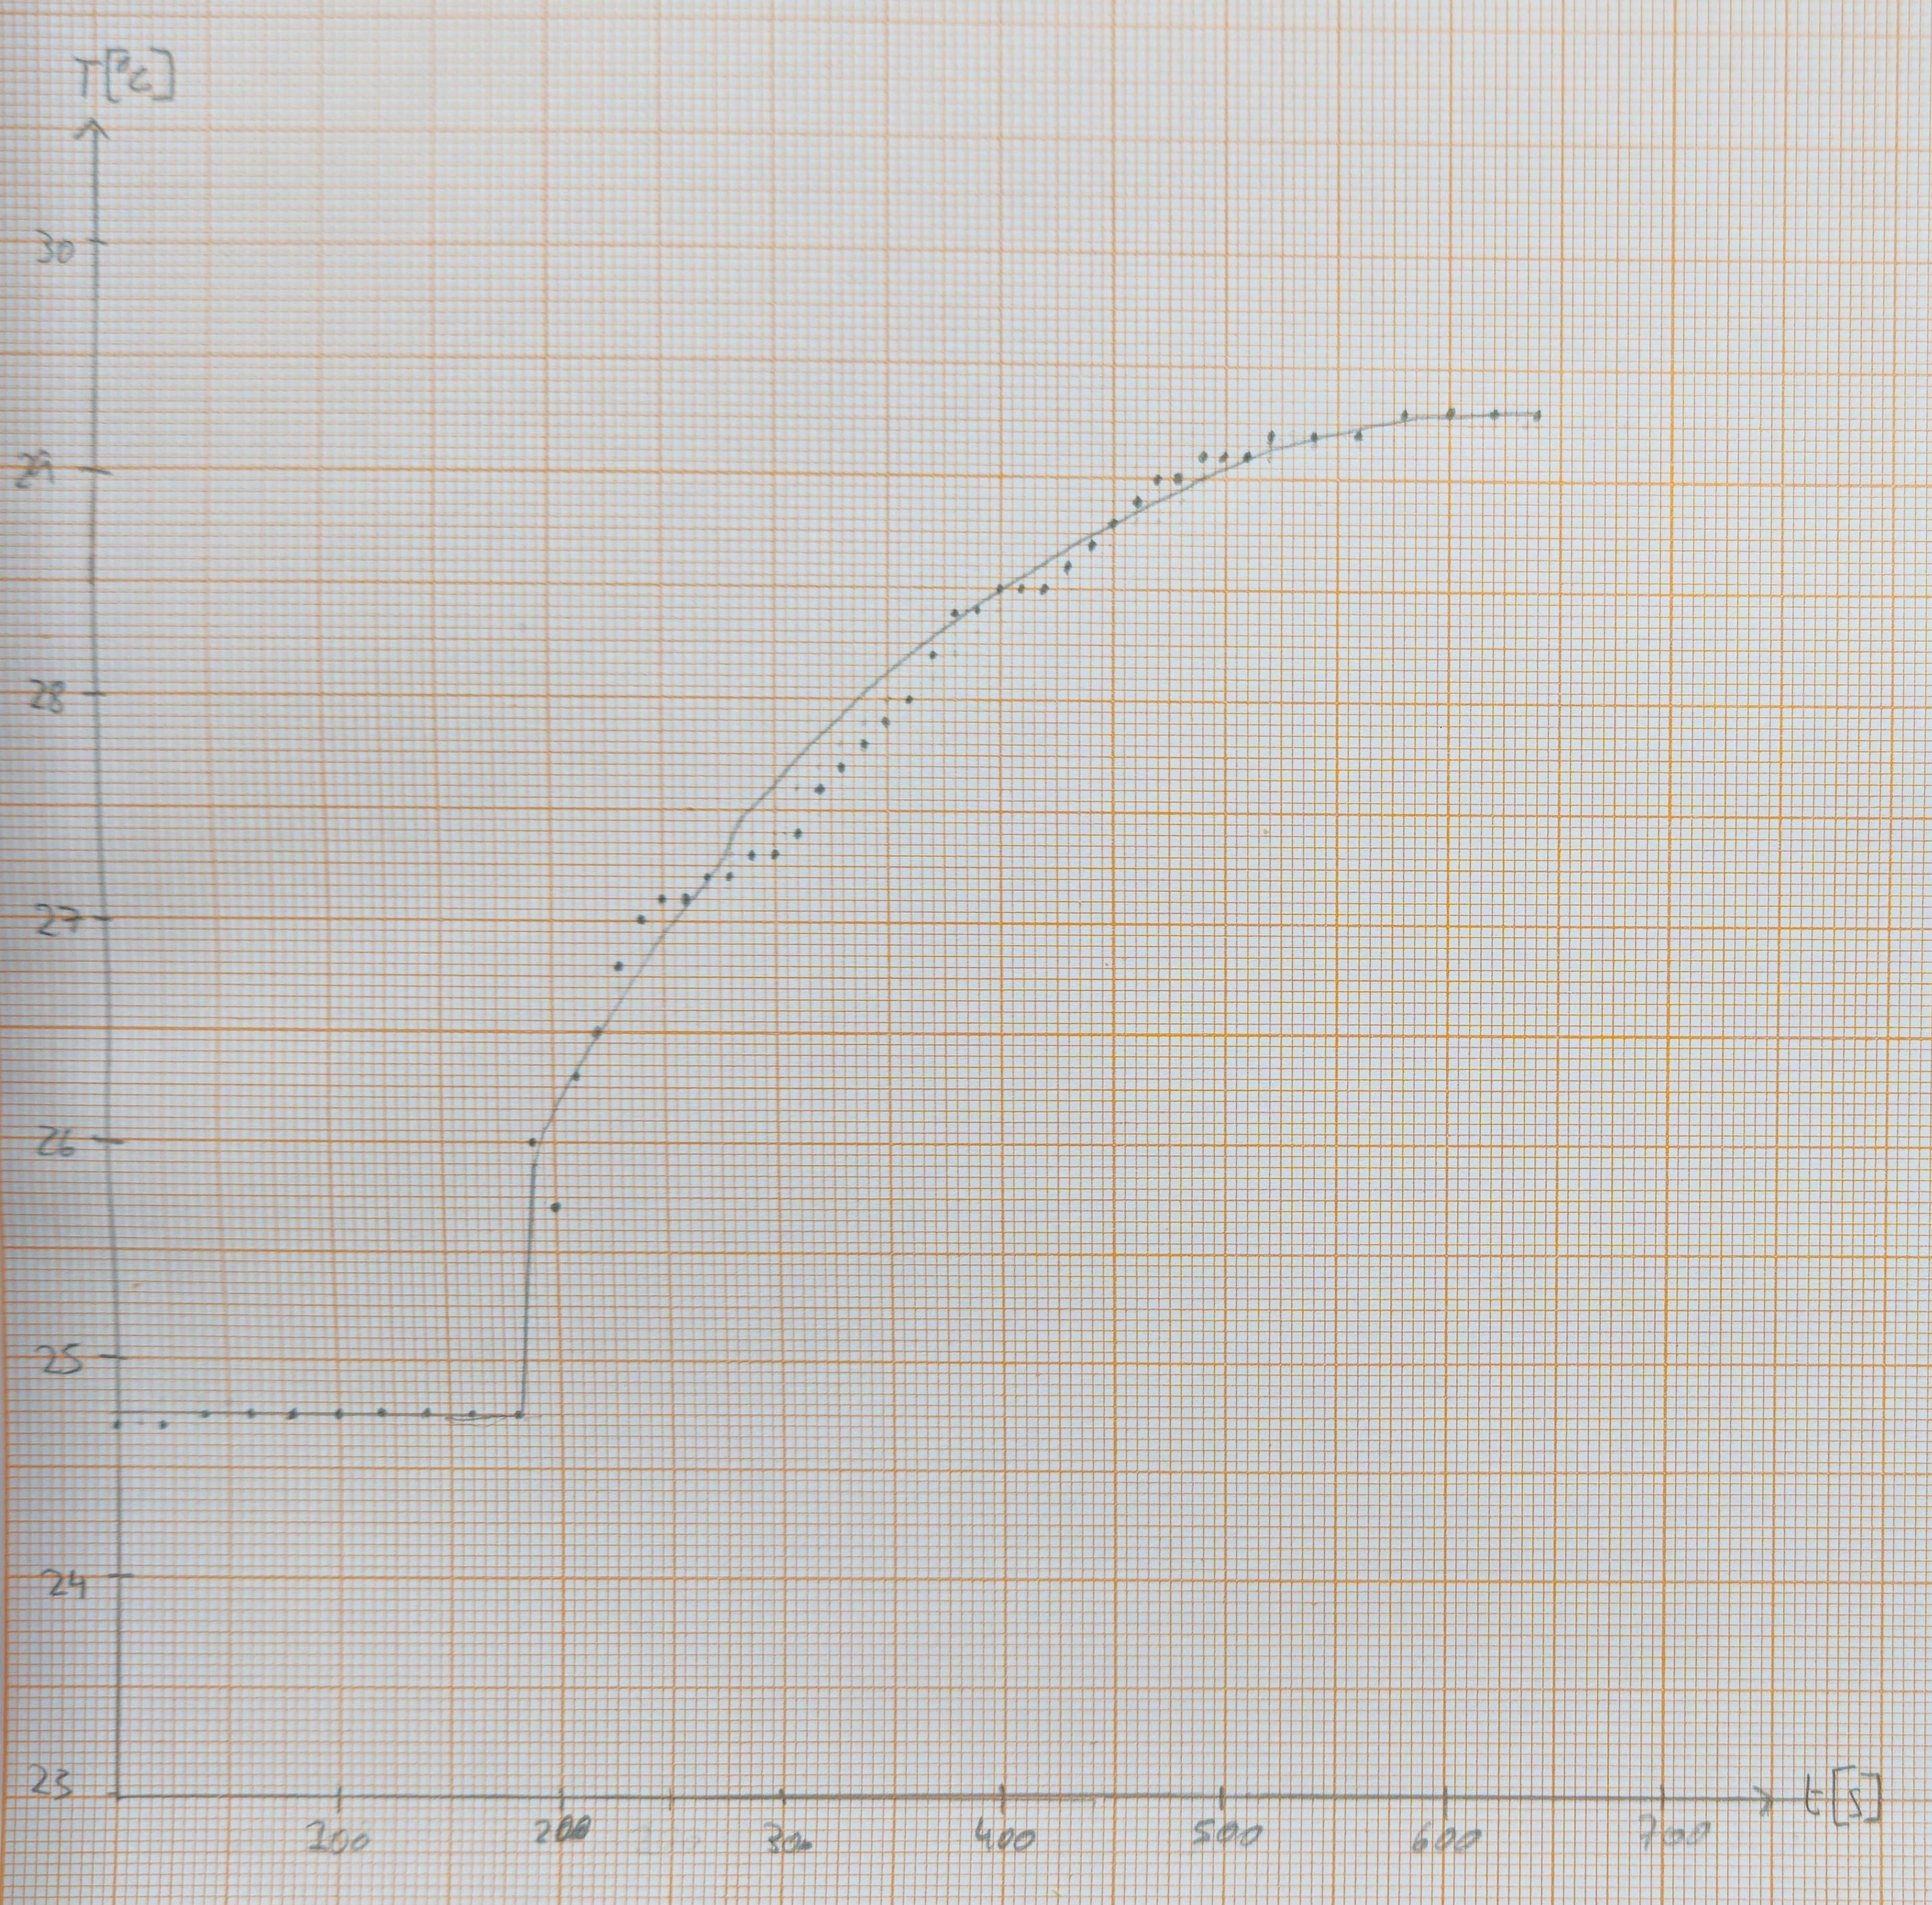
\includegraphics[width=\textwidth]{fotocalorimetro/acquaoggetto.jpg}
    \caption{Grafico di $T(t)$ del calore specifico dell'ottone }
\end{figure}
\FloatBarrier

\newpage
\subsection{Calore Latente del Ghiaccio}
\begin{figure}[!ht]
    \centering
    \includegraphics[width=\textwidth]{fotocalorimetro/acquaghiaccio.jpg}
    \caption{Grafico di $T(t)$ del calore latente del ghiaccio}
\end{figure}

\end{document}
